\chapter[Resultados]{Resultados}

Este capítulo apresenta os resultado obtido com a aplicação dos exemplos
 de uso descritos no Capítulo \ref{exemplos_de_uso}.

Para melhor organização do trabalho, os resultados serão apresentados em seções,
 que correspondem à métodos correlacionados.

\section{Guardas de Inclusão}

As tabelas que contém o detalhamento das execuções dos experimentos se encontram
 no Apêndice \ref{guardas_de_inclusao_apendice}.
 A Tabela \ref{tab:resutados_guards_de_inclusao}
sintetiza as médias destes resultados, e a Figura \ref{benchmark_guardas_de_inclusao} apresenta os mesmos dados, em forma
visual. Os tempos são dados em segundos, e os métodos aplicados foram abreviados com as seguintes siglas:

\begin{description}
    \tiny
    \item [GIE:] Guarda de Inclusão Externa
    \item [GII:] Guarda de Inclusão Interna
    \item [PO:]  Pragma Once
    \item [GIIPPO:] Guarda de Inclusão Interna Primeiro que Pragma Once
    \item [POPGII:] Pragma Once Primeiro que Guarda de Inclusão Interna
    \item [GIEPPO:] Guarda de Inclusão Externa e Pragma Once
    \item [RGI:] Redundancia de Guarda de Inclusão
\end{description}

\begin{table}[!ht]
\centering
\caption{Resultados das Guardas de Inclusão}
\label{tab:resutados_guards_de_inclusao}
\begin{tiny}
\begin{tabular}{lp{1cm}p{1cm}p{1cm}p{1cm}p{1cm}p{1cm}p{1cm}p{1cm}}
& \multicolumn{7}{c}{\textbf{Tempo médio de compilação (em segundos)} } \\
\textbf{Sistema Operacional} & \textbf{GIE} & \textbf{GII} & \textbf{PO} &
\textbf{GIIPPO} & \textbf{POPGII} & \textbf{GIEPO} & \textbf{RGI} \\ \toprule
 Linux & 0,2851     & 0,2851  & 1,2127    & 1,3179    & 1,2311  & 1,2477     & 0,1611 \\
 Mac OS Yosemite & 0,8482 & 0,8149 & 1,0031  & 1,0139  & 0,9511  & 0,9097  & 0,5668  \\ 
 Windows 7 & 2,4015 & 2,3954 & 4,2161 & 4,2611 & 4,3152 & 4,2621  & 2,1471 \\
\bottomrule
\end{tabular}
\end{tiny}
\end{table}

\begin{figure}[!h]
    \centering
        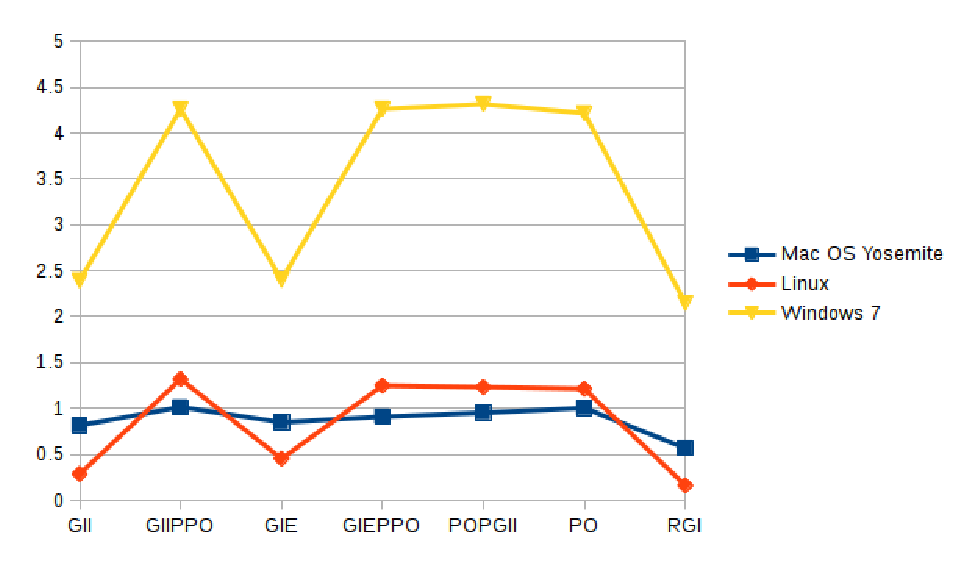
\includegraphics{figuras/graficos/benchmark.eps}
    \caption{Dados coletados dos scripts de Guardas de Inclusão}
    \label{benchmark_guardas_de_inclusao}
\end{figure}

De acordo com dados apresentados, pode-se observe que, para os experimentos em questão, todos os métodos que utilizam a diretiva 
\texttt{\#pragma once} atigiram tempo de compilação superior em relação aos métodos a utilizam, independente do sistema operacional em questão.
Dentre os métodos que não utilizaram esta diretiva, o método \textbf{RGI} foi o que resultou em menor tempo médio de compilação.

Em relação aos sistemas operacionais listados, o Mac OS Yosemite apresentou a menor variação dentre os diferentes métodos, apresentado comportamento 
aproximadamente linear (com média 0,8725 e desvio padrão de 0,1424, o que corresponde a 16\% de variação em torna da média, contra 61\% e 28\% obtido
no Linux e Windows, respectivamente).  No Windows 7, o tempo de compilação dos métodos foi, na maior parte dos métodos, de 3 a 4 vezes maior que nos outros sistemas operacionais. 


\section{Métodos que envolvem a edição do código fonte}

O primeiro método avaliado, que evolve a edição do código fonte, foi a guarda de inclusão \texttt{\#pragma once} (apresentada na Seção \ref{include_guards_section}). Este método foi aplicado em todos os 5 projetos selecionado, e os tempos médios de compilação são apresentados na Tabela \ref{tab:pragma}.

\begin{table}[!ht]
\tiny
\centering
\caption{Resultados do \texttt{\#pragma once}}
\label{tab:pragma}
\begin{tabular}{lccccccccc}
& \multicolumn{6}{c}{\textbf{Tempo médio de compilação (em segundos)} } \\
\textbf{Projeto} & \multicolumn{3}{c}{\textbf{Linux}} & \multicolumn{3}{c}{\textbf{Mac OS Yosemite}} & \multicolumn{3}{c}{\textbf{Windows 7}} \\ 
& \textbf{Sem } & \textbf{Com }  & \textbf{Redução (\%)} & \textbf{Sem } & \textbf{Com }  & \textbf{Redução (\%)} & \textbf{Sem } & \textbf{Com }  & \textbf{Redução (\%)} \\
\toprule
Aseprite & 2362 &  2357 & 0,021     & 769  & 772 &   - &  2441 & 2317 & 5,07 \\
iRecoveryplusplus & 1,16 & 0,86     & 25,9 & 2,85 & 2,92 & - & 4,88     & 5,02 & - \\
Pencil & 455  &  459  &  - &  353   & 346  & 1,98 &  530      & 529 &  0,18 \\
Sudoku & 22   &  22   &  - &  38    & 38   & -  &  32 & 29 & 9,37 \\ 
Qcad   & 3923 &  3841 &  2,09  &  3729  & 3290 & 11,77   & - & -  & - \\ 
\end{tabular}
\end{table}

Para os projetos selecionados, o impacto desta técnica não se mostrou relevante, pois em várias configurações não houve sequer ganho em relação ao tempo médio e, nos casos onde
houve ganho, a porcentagem foi muito baixa (exceto no caso do iRecoveryplusplus no Linux, com 25\% de ganho, mas o tempo de compilação do projeto já era muito baixo, o que afeta diretamente na proporção ganho).

O segundo método que envolve a edição de código fonte foi a técnica de declaração implicita de estrutura (encontrada na Seção \ref{forward_declaration_section}). Este método foi aplicado apenas em 2 projetos, pois os outros projetos já possuiam esta técnica. A Tabela \ref{tab:forward_declaration} apresenta  os tempos médios de compilação produzidos durante a coleta de dados.

\begin{table}[!ht]
\tiny
\centering
\caption{Resultados da declaração implicita de estrutura}
\label{tab:forward_declaration}
\begin{tabular}{lccccccccc}
& \multicolumn{6}{c}{\textbf{Tempo médio de compilação (em segundos)} } \\
\textbf{Projeto} & \multicolumn{3}{c}{\textbf{Linux}} & \multicolumn{3}{c}{\textbf{Mac OS Yosemite}} & \multicolumn{3}{c}{\textbf{Windows 7}} \\ 
& \textbf{Sem } & \textbf{Com }  & \textbf{Redução (\%)} & \textbf{Sem } & \textbf{Com }  & \textbf{Redução (\%)} & \textbf{Sem } & \textbf{Com }  & \textbf{Redução (\%)} \\
\toprule
iRecoveryplusplus &  1,17  &   0,9   & 23,7  &   2,85  &  2,7   & 5,26 &  4,97 & 4,3   & 13,48 \\
Sudoku            & 22,21  & 20,63   & 7,11  &  38.42  & 36.26  & 5,62  & 32,72 & 27,97 & 14,51  \\ 
\end{tabular}
\end{table}

Para os projetos avaliados o impacto desta técnica reduziu o tempo de compilação, no entanto não se mostrou tão relevante, uma vez que o tempo de redução máximo atingido foi de 23,7\% ( no qual este projeto possui um tempo de compilação muito baixo e com uma variação muito alta levando a uma perda de proporção) no Linux e as outras ocorrencias reduziram menos de 15\% do tempo de compilação. 
O terceiro método avaliado que envolve a edição de código foi a implementação do ponteiro de declaração privada encontrado no Seção \ref{Pimpl_Idiom}. Aplicando esta técnica a Tabela \ref{tab:pimpl} foi elaborada com os tempos médios de compilação dos 3 projetos que foram alterados utilizando a técnica.

\begin{table}[!ht]
\tiny
\centering
\caption{Resultados da aplicação ponteiro de implementação privada }
\label{tab:pimpl}
\begin{tabular}{lccccccccc}
& \multicolumn{6}{c}{\textbf{Tempo médio de compilação (em segundos)} } \\
\textbf{Projeto} & \multicolumn{3}{c}{\textbf{Linux}} & \multicolumn{3}{c}{\textbf{Mac OS Yosemite}} & \multicolumn{3}{c}{\textbf{Windows 7}} \\ 
& \textbf{Sem } & \textbf{Com }  & \textbf{Redução (\%)} & \textbf{Sem } & \textbf{Com }  & \textbf{Redução (\%)} & \textbf{Sem } & \textbf{Com }  & \textbf{Redução (\%)} \\
\toprule
iRecoveryplusplus  &   1,17   &  0,91   & 22,22   & 2,85  & 2,70   & 5,26  & 4,97 & 4,83 & 2,81 \\ 
Pencil             &   455    &  454    & 0,22    & 353   & 353    & -     & 530 & 520   & 1,88 \\
Sudoku             &   22,21  & 21,39   & 3,69    & 38,42 & 37,82  & 1,56  & 32,72 & 28,78 & 12,04 \\ 
\end{tabular}
\end{table}

Para os projetos avaliados esta técnica impactou na redução do tempo de compilação, no entanto entanto em projetos com tempo de compilação grande como no \textit{Pencil}, que demorou cerca de 7 a 8 minutos para compilar, a redução foi de 0,22\%, mostrando-se que esta técnica apesar de reduzir a compilação não possui um impacto relevante na compilação de um projeto.

Por fim, os dados detalhados de todos os experimentos com métodos que envolvem a edição do código fonte estão no Apêndice \ref{metodos_codigo_apendice}.



\section{Métodos que envolvem a parametrização do \textit{build}}


O primeiro método avaliado na parametrização de \textit{build} é o
 método que utiliza flags de otimização,
 apresentado na Seção \ref{Otimizacao_de_baixo_nivel}. Este método foi
 aplicado em todos os 5 projetos selecionados. A Tabela 
\ref{tab:flags_de_otimização:linux} apresenta os resultados coletados no ambiente linux.
 Vale ressaltar que em todos os projetos a o gerador de makefile coloca por padrão a \textit{flag} \texttt{-O2} no makefile.
 
\begin{table}[!ht]
\tiny
\centering
\caption{Resultados com flags de otimização no Linux}
\label{tab:flags_otimizacao:linux}
\begin{tabular}{lccccccccc}
& \multicolumn{6}{c}{\textbf{Tempo médio de compilação (em segundos)} } \\
 \textbf{Projeto}& \textbf{-O}  & \textbf{-O0}   & \textbf{-O2} & \textbf{-O3} & \textbf{-Os} & \textbf{-Ofast} & \textbf{-Og} & \textbf{Melhor Redução (\%)}\\ \toprule
Aseprite            & 2274  & 2073          & 2357  & 2412  & 2246              & \textbf{705} & 2253 & 70 \\
iRecoveryplusplus   & 1,04  & \textbf{0,89} &  1,17 & 1,12  & 0,90              & 1,13  & 1,03 & 23,93 \\
Pencil              & 456   & 454           &  455  & 455   & \textbf{453}      & 455   & 455 & 0,44\\
Sudoku              & 22,23 & 22,51         & 22,21 & 21,92 & \textbf{19,65}    & 21,92 & 22,08 &  11,53 \\ 
Qcad                & 3919  &  3925         &  3923 & 3919  & \textbf{3886}     & 3922  & 3937 & 0,94  \\ 
\end{tabular}
\end{table}


No ambiente linux esta técnica teve um ganho maior no projeto \textit{Aseprite} com a utilização da \textit{flag} \texttt{-Ofast} com uma redução de 70\%  do tempo de compilação. No entanto vale lembra que este projeto utiliza o gerador de makefile cmake, e os outros projetos em sua maioria utiliza o qmake. De maneira geral a maioria dos projetos tiveram redução utilizando a \textit{flag } \texttt{-Os}.

 Com o ambiente Mac OS Yosemite a Tabela \ref{tab:flags_otimizacao:mac_os} apresenta os resultados do tempo de compilação médio obtido utilizando esta técnica. Neste ambiente foi possível utilizar utilizar o método nos 5 projetos, no entanto a \textit{flag} \texttt{-Og} não foi utilizada devido ao \textit{back-end} do LLVM não suportar.

\begin{table}[!ht]
\tiny
\centering
\caption{Resultados com flags de otimização no Mac OS Yosemite}
\label{tab:flags_otimizacao:mac_os}
\begin{tabular}{lccccccccc}
& \multicolumn{6}{c}{\textbf{Tempo médio de compilação (em segundos)} } \\
 \textbf{Projeto}& \textbf{-O}  & \textbf{-O0}   & \textbf{-O2} & \textbf{-O3} & \textbf{-Os} & \textbf{-Ofast} & \textbf{Melhor Redução (\%)}\\ \toprule
Aseprite            & 775   &  592 &  769   & 795            & 708 & \textbf{209}  & 72,82 \\ 
iRecoveryplusplus   & 2,90  & \textbf{2,57} & 2,85           & 2,83 &  2,76  & 2,86  & 9,82 \\ 
Pencil              & 353   & \textbf{352}  & 353            & 353  & 364 & 356 &  0,39 \\ 
Sudoku              & 38,36 & 38,50 & 38,42 & \textbf{38,32} & 39,38 & 38,34 & 0,26  \\ 
Qcad                & 3795  & \textbf{3079} & 3729           & 3737 & 3793  & 3786 &  17,43  \\ 
\end{tabular}
\end{table}

Para este ambiente o projeto \textit{Aseprite} também obteve o maior ganho 
 utilizando o \textit{flag} \texttt{-OFast}. Vale resaltar que como dito anteriormente este
 projeto foi criado utilizando o gerador de makefile cmake, diferente dos outros projetos.
 Avaliando o impacto em todos os projetos a \textit{flag} \texttt{-O0} obteve um maior redução.


No ambiente Windows 7 a Tabela \ref{tab:flags_otimizacao:windows} apresenta o tempo
 de compilação médio utilizando apenas 4 projetos selecioados, pois dito anteriormente
 na Seção \ref{impedimentos_durante_a_coleta} o projeto \ref{Qcad} não pode ser instalado
 devido a falta de dependências neste ambiente.

\begin{table}[!ht]
\tiny
\centering
\caption{Resultados com flags de otimização no Windows 7}
\label{tab:flags_otimizacao:windows}
\begin{tabular}{lccccccccc}
& \multicolumn{6}{c}{\textbf{Tempo médio de compilação (em segundos)} } \\
 \textbf{Projeto}& \textbf{-O}  & \textbf{-O0}   & \textbf{-O2} & \textbf{-O3} & \textbf{-Os} & \textbf{-Ofast} & \textbf{-Og} & \textbf{Melhor Redução (\%)}\\ \toprule
Aseprite            &  2254     & 2092          & 2441   & 2550  & 2231          & \textbf{620}  & 2184  & 74,6  \\ 
iRecoveryplusplus   & 4,58      & 4,65          & 4,97   & 5,17  & \textbf{4,53} & 4,95          &  4,85 &  8,85 \\ 
Pencil              & 516       & \textbf{501}  & 530    & 534   & 522           & 539           & 513   & 5,47 \\ 
Sudoku              & 31,15     & \textbf{29,29} & 32,72 & 35,28 & 31,41         & 35,69         & 30,11 & 16,98 \\ 
\end{tabular}
\end{table}

Analisando os resultados dos projetos avaliados, o projeto Aseprite foi o obteve o maior
 ganho utilizando a \textit{flags} \texttt{-Ofast}. No entanto de uma maneira geral
 a \textit{flag} \texttt{-O0} obteve o maior ganho na maioria dos projetos, exceto no projeto iRecoveryplusplus que possui o menor tempo de compilação dentre todos os projetos analisados.


Após a parametrização utilizando \textit{flags} de otimização foi realizada a
 parametrização utilizando \textit{flags} de processamento paralelo com a ferramenta make.
Esta técnica foi mensionada na Seção \ref{Makefile_section} e foi possível utilizar todos os projetos selecionados.
 A Tabela \ref{tab:flags_processamento_paralelo:linux} apresenta os dados coletados utilizando este método no ambiente Linux, e demostra o tempo médio de compilação dos projetos utilizando cada uma das \textit{flags}.

\begin{table}[!ht]
\tiny
\centering
\caption{Resultados com flags de processamento paralelo no Linux}
\label{tab:flags_processamento_paralelo:linux}
\begin{tabular}{lccccccc}
& \multicolumn{4}{c}{\textbf{Tempo médio de compilação (em segundos)} } \\
\textbf{Projeto} & \textbf{sem flag} & \textbf{-j 2} & \textbf{-j 4} & \textbf{-j 6} & \textbf{-j 8} & \textbf{-j10} &  \textbf{Melhor Redução (\%)} \\ \toprule
Aseprite            & 2357  & 1390              & \textbf{1229} & 1479  & 1695      & 1439          & 47,85  \\ 
iRecoveryplusplus   & 1,17  & \textbf{1,11}     &  1,12         & 1,13  & 1,13      & 1,12          & 5,13 \\ 
Pencil              & 455   & 271               & \textbf{242}  & 257   & 284       & 288           &  46,81 \\ 
Sudoku              & 22    & 13                & 13            & 13    & 14        & \textbf{10}   & 54,54  \\ 
Qcad                & 3923  & 2437              & \textbf{2301} & 2323  & 1603      & 1557          & 41,34 \\ 
\end{tabular}
\end{table}

No ambiente Linux ao utilizar qualquer uma das \textit{flags} o tempo de compilação é
 reduzido em mais de 40\% em todos os projetos. De maneira geral o uso
 da \textit{flag} \texttt{-j 10} não necessáriamente é o
 que impacta na maior redução do tempo de compilação, pois nos casos
 apresentados a maior parte dos projetos tiveram o menor
 tempo de compilação utilizando a \textit{flag} \texttt{-j 4}.

Para o ambiente Mac OS Yosemite a Tabela \ref{tab:flags_processamento_paralelo:mac_os} apresenta os resultados obtidos utilizando esta técnica. Todos os projetos selecionados foram utilizados.

\begin{table}[!ht]
\tiny
\centering
\caption{Resultados com flags de processamento paralelo no Mac OS Yosemite}
\label{tab:flags_processamento_paralelo:mac_os}
\begin{tabular}{lccccccc}
& \multicolumn{4}{c}{\textbf{Tempo médio de compilação (em segundos)} } \\
\textbf{Projeto} &  \textbf{sem flag} & \textbf{-j 2} & \textbf{-j 4} & \textbf{-j 6} & \textbf{-j 8} & \textbf{-j10} &  \textbf{Melhor Redução (\%)} \\ \toprule
Aseprite          & 769   & 576   & 575   & \textbf{288}  & 578 & 571      &  62,54 \\ 
iRecoveryplusplus & 2,85  & 2,50  & 2,73  &  2,50 &  2,41 &  \textbf{2,33} & 18,24\\ 
Pencil            & 353   & 279   & 275   & 282 & 276     & \textbf{265}   & 24,92 \\ 
Sudoku            &  38   & 28,27 & 28,17 & 27,97 & 28,31 & \textbf{27,94} & 26,47 \\ 
Qcad              & 3729  & 3596  & 3685  & 3745 & 3422   & \textbf{3103}  & 16,78 \\ 
\end{tabular}
\end{table}

No ambiente Mac OS Yosemite esta tecnica apresentou resultados diferentes do ambiente Linux.A \textit{flag} \texttt{-j 10} resultou no menor tempo de compilação na maioria dos projetos.No entanto a redução neste ambiente não passou de 27\%, exceto no projeto \textit{Aseprite} que utilizando a \textit{flag} obteve uma redução maior que 60\%.


Com a utilização desta tecnica no ambiente Windows 7 a Tabela \ref{tab:flags_processamento_paralelo:windows} apresenta os resultados obtidos.
Apenas o projeto Qcad não foi possível ser utilizado neste ambiente, devido a necessidade de uma dependência de ambiente como mostrado na Seção \ref{impedimentos_durante_a_coleta}.


\begin{table}[!ht]
\tiny
\centering
\caption{Resultados com flags de processamento paralelo no Windows 7}
\label{tab:flags_processamento_paralelo:windows}
\begin{tabular}{lccccccc}
& \multicolumn{4}{c}{\textbf{Tempo médio de compilação (em segundos)} } \\
\textbf{Projeto} & \textbf{sem flag} & \textbf{-j 2} & \textbf{-j 4} & \textbf{-j 6} & \textbf{-j 8} & \textbf{-j10} &  \textbf{Melhor Redução (\%)} \\ \toprule
Aseprite            & 2441      & 1140      & 1093      & \textbf{1005}     & 1083 & 1022  &  58,82  \\ 
iRecoveryplusplus   & 4,97      & 4,99      &  5,02     & 5,11              & 5,01 & \textbf{4,94} & 0,60 \\ 
Pencil              & 530       & 262,35    & 259,95    & \textbf{258,90}   & 259,15 & 266,47  & 51,15 \\ 
Sudoku              & 32,72     & 17,32     & 17,84     & \textbf{16,57}    & 18,43 & 18,14 & 49,36 \\ 
\end{tabular}
\end{table}

Com os projetos selecionados, a maioria dos projetos apresentou uma redução superior a 50\%  utilizando a \textit{flag} \texttt{-j 6}, exceto no iRecoveryplusplus em que seu tempo de compilação é muito baixo e sendo assim a redução foi pouco relevante.


Por fim as Tabelas apresentadas na Seção \ref{metodos_ferramentas_aplicados_a_um_projeto_template} foram preenchidas e estão disponíveis no Apêndice localizados na Seção \ref{parametrizacao_apendice}.


\section{Métodos que envolvem o uso de ferramentas externas}


Com a utilização de ferramentas externas o \textit{linker} \textit{gold}
 foi utilizado apenas no ambiente Linux, como exposto na Seção
 \ref{ferramentas_de_otimizacao}. A Tabela \ref{tab:gold} apresenta
 os tempos médios da compilação dos 5 projetos selecionados.

\begin{table}[!ht]
\tiny
\centering
\caption{Resultados com uso do \textit{linker gold}}
\label{tab:gold}
\begin{tabular}{lccc}
& \multicolumn{3}{c}{\textbf{Tempo médio de compilação (em segundos)} } \\
\textbf{Projeto} & \multicolumn{3}{c}{\textbf{Linux}} \\ 
& \textbf{Sem } & \textbf{Com }  & \textbf{Redução (\%)} \\
\toprule
Aseprite            & 2357  & 2270      & 3,69 \\
iRecoveryplusplus   & 1,17  & 1,00      & 14,52 \\
Pencil              & 455   & 457,37    & - \\ 
Sudoku              & 22    & 21,17     & 3,77  \\
Qcad                & 3923  & 3847      & 1,94 \\
\end{tabular}
\end{table}

Utilizando esta ferramenta na maioria dos projetos o tempo de
 compilação é considerado irrelevante pois reduzido em menos de 4\% nos casos em que houve redução,
 exceto no projeto iRecoveryplusplus que possui o tempo de compilação
 muito baixo e então os ganhos são apresentados de maneira desproporcional.

A segunda ferramenta \textit{ccache}, que é detalhada na Seção \ref{ferramentas_de_otimizacao},
foi utilizada em todos os 5 projetos selecionais. A Tabela \ref{tab:ccache} apresenta os
 dados coletados tendo como médida o tempo de compilação médio em segundos.


\begin{table}[!ht]
\tiny
\centering
\caption{Resultados com uso da ferramenta \textit{ccache}}
\label{tab:ccache}
\begin{tabular}{lccccccccc}
& \multicolumn{6}{c}{\textbf{Tempo médio de compilação (em segundos)} } \\
\textbf{Projeto} & \multicolumn{3}{c}{\textbf{Linux}} & \multicolumn{3}{c}{\textbf{Mac OS Yosemite}} & \multicolumn{3}{c}{\textbf{Windows 7}} \\ 
& \textbf{Sem } & \textbf{Com }  & \textbf{Redução (\%)} & \textbf{Sem } & \textbf{Com }  & \textbf{Redução (\%)} & \textbf{Sem } & \textbf{Com }  & \textbf{Redução (\%)} \\
\toprule
Aseprite & 2357,87 & 540,58 & 77,07 & 769,16 & 209,82 & 72,72  & 2441,38 & 761,73  & 68,80 \\ 
iRecoveryplusplus & 1,17 & 1,14 & 2,56    & 2,85 & 2,63 & 7,71  & 4,97 & 5,04 & -  \\ 
Pencil & 455  & 173 & 61,98 & 353 & 104  & 70,54  & 530  & 181  & 65,85 \\ 
Sudoku & 22 & 4 & 81,81  & 38 & 7 & 81,58  & 32 & 8  &  75    \\ 
Qcad  & 3923 & 1823 & 53,53 & 3729 & 664 & 82,19 &  -  & -  & -  \\ 
\end{tabular}
\end{table}


O uso da ferramenta ccache proprocionou uma redução significativa na
 maioria dos projetos, e com maior impacto em projetos grandes.
 O projeto iRecoverypluplus possui os menores tempos de redução devido
 ao mesmo possuir o menor tempo médio de compilação.
 Os gráficos \ref{grafico_ccache_linux}, \ref{grafico_ccache_mac_os} e
 \ref{grafico_cache_windows} apresentados no Apêndice proporcionam uma
 melhor visualização destes dados. 

Por fim os dados para uma visualização de dados mais detalhados da utilização destas ferramentas é apresentado no Apêndice \ref{uso_de_ferramentas_externas_apendice}.
